\documentclass[a5paper,10pt]{article}

\usepackage[utf8]{inputenc}
\usepackage[magyar]{babel}
\usepackage[T1]{fontenc}
\usepackage{amsmath}
\usepackage{amssymb}
\usepackage[margin=20mm]{geometry}
\usepackage{graphicx}
\usepackage{lmodern}
\usepackage{indentfirst}
\usepackage{hyperref}
\usepackage{accsupp}
\frenchspacing

\begin{document}


% ------------------------------------------------------------------------------


\renewcommand{\thefootnote}{\fnsymbol{footnote}}

\begin{center}{\Large\bf
Rászoruló embertársaink megsegítése\\[1mm] szociális média felületeken
}\end{center}
\vspace*{1mm}
%
\begin{center}{\large\bf\noindent
Raven Sztupák Szilárd Zsolt
}\\[3mm]
%
Eötvös József Collegium{\footnote[1]{2004--2009}}
%
\\[2mm]\texttt{
zsolt@raven.scot}
\end{center}
\vspace*{7mm}
\renewcommand{\thefootnote}{\arabic{footnote}}


% ------------------------------------------------------------------------------


\section{Bevezetés}

Az egyetem elvégzése után számos lehetőség adódik a volt hallgatóknak, hogy mit kezdjenek életükkel. Vannak, akik a szakmán kívül helyezkednek el, mások maradnak az egyetem csábító közelségében. Elég gyakori az is, hogy a korporét élet GDP termelési mutatói veszik le lábukról az embereket, akik emiatt úgy döntenek, hogy a magánszektorban folytatják pályafutásukat. Függetlenül attól, hogy milyen életpályát választunk, a megszerzett tudásunkkal ne legyünk önzők, és ahol tudunk, próbáljunk segíteni felebarátainkon.

\bigskip

Vannak erre kifejezetten szakosodott nemzetközi közhasznú szervezetek. Egyik ilyen a CodeBar\cite{codebar}, ami a technológiai szektorban alulreprezentált embertársainknak segít azzal, hogy keres nekik tapasztaltabb mentorokat a problémáik megoldásában. Sokáig volt Budapesten is aktív közösségük, azonban ez sajnos 2019 körül önkéntesek hiányában elapadt. Segítő szándékú fejlesztők jelentkezését nemzetközi szinten azonban szivesen várják, akár online, távmunkában is lehet nekik havonta 1-2 óra ráfordítással besegíteni. A szerző emellett természetesen nagyon reméli, hogy idővel a budapesti közösség is újra aktív lesz.

\bigskip

A másik hasonló nemzetközi kezdeményezés pedig a MigraCode\cite{migracode}, mely menekülteknek, és hátrányos szociális helyzetből származó embereket segít programozni tanítani. Nekik sajnos nincs kirendeltségük Magyarországon, de több országban aktív szervezetük is szívesen várja a távmunkában segíteni szándékozó jelölteket!

\bigskip

Azonban nem ez az egyetlen módja a segédkezésnek. Ha valaki szemfüles, és odafigyel, akkor szociális média felületeken is könnyedén találhat oltalomra szoruló illetőket. Az alábbi cikkben három példán keresztül mutatom be hogyan tudunk embertársaink támogatására sietni, ha szükségük lenne rá!

% ------------------------------------------------------------------------------

\section{Kossuth Lajos azt üzente}

\texttt{sztivan} felhasználónevű Tumblr felhasználó egy hűvős februári napon úgy érezte, hogy egy fontos információt szeretne a világról megtudni. Ez az információ pedig nem más, mint amit a \ref{sztivan:question}. ábrán ábrázolt képernyőmentés ábrázol\cite{sztivan}.

\begin{figure}[!htbp]
    \centering
    \BeginAccSupp{method=plain,Alt={Az irreleváns kérdés, amire megpróbálnám keresni a választ, ha végtelenül sok fölösleges időm volna: hol található Magyarországon a hely, ami a legtávolabb van egy Kossuth utcától?}}%
    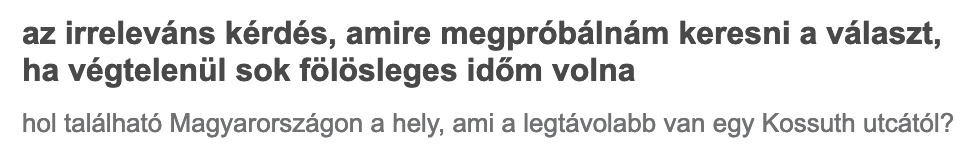
\includegraphics[width=\textwidth]{images/kossuth_kerdes.png}
    \EndAccSupp{}%
    \caption{Problémafelvetés}
    \label{sztivan:question}
\end{figure}

Ez pontosan az a fajta kérdés ahol a több évnyi Eötvös Collegium-ban szerzett tapasztalatomat alkalmazni tudom. Aktív szociális életet élő lényként a Földrajz-Földtudomány műhely tagjaival gyakran szerveztünk közös programokat, ami során megismerkedtünk egyik kedvenc\footnote{gy.k.: gyűlölt} foglalkozásukkal, ami nem más, mint térképek digitalizálása. Ez a nagyszintű precizitást és monotontűrést igénylő feladat lehetővé teszi, hogy régi, papír alapú térképeken szereplő adatokat digitális eszközökkel kezeljünk, rajtuk különféle lekérdezéseket futtassunk le. Ezúton is szeretném köszönetemet kifejezni azokkal szemben, akik ezeket a tevékenységeket önerőből, gyakran anyagi kompenzáció nélkül elvégezték, és végül munkájuk eredményét ingyen elérhetővé tették a világhálón, főleg mert így ezt már nem nekem kell megtenni.

\bigskip

Nemzetközi viszonylatban a legismertebb ilyen digitalizációs projekt az EC Informatikai Műhelyével egyidős OpenStreetMap\cite{osm}, mely célja egy egész bolygót lefedő, ingyenes térképészeti adatbázis létrehozása. Hasonló projekt a szintén 2004 óta létező magyar Turistautak\cite{turistautak} is, mely Magyarország és a környező országok turistaútjainak feltérképezését tűzte ki céljául. A két projekt sokáig egymás konkurrenciájaként üzemelt, többek között a különböző licenszfeltételekenek köszönhetően: míg a Turistautak térképének böngészése kizárlóag non-profit céllal volt engedélyezett, addig az OpenStreetMap adatait kereskedelmi célokra is fel lehetett használni. 2015-ben történt egy változás, amikor a Turistautak szerkesztősége szintén teljesen szabaddá tette az adatokat, ami után a két projekt adatbázisa  összefésülésre került. Ennek eredményeképpen az OpenStreetMap Magyarországgal kapcsolatos része is élvezhette a több évnyi, önkéntes digitalizációs munka eredményét.

\bigskip

Ez nekünk pont kapóra jön, mert a kérdés megválaszolásához szükségünk lesz Magyarország összes Kossuth utcájának a listájára, amit az OSM adatbázisából fogjuk beszerezni. Számos eszköz létezik, hogy az OSM adatait saját számítógépünkön kezeljük, az \texttt{osmosis}, valamint az \texttt{osmconvert} parancsssoros, míg például a \texttt{QGis} grafikus feldolgozást tesz lehetőve. Mindegyik említett ezköz ingyenes, nyílt forráskódú. A \ref{osmextract}. ábrán látható módon fogjuk őket használni, először, hogy az egész Magyarországot tartalmazó adatsort leszűrjük csak a nevesített utakra (amelyek az OSM rendszerben \texttt{highway} jelzéssel vannak ellátva), majd utána hogy ebből a szűrt adatokból egy CSV állományt nyerjünk ki a Kossuth utcák középpontjának GPS koordinátáival.

\begin{figure}[!htbp]
    \centering
    \begin{verbatim}$ osmosis –read-pbf-fast hungary.osm.pbf
    file=“hungary.osm.pbf” –way-key keyList=highway
    –way-key keyList=name –used-node –tag-filter
    reject-relations –write-xml file=“hungary-roads.osm”
$ osmconvert hungary-roads.osm –all-to-nodes
    –csv=“@id @lon @lat name” –csv-headline | grep -i
    kossuth > streets.csv\end{verbatim}
    \caption{Kossuth utcák adatainak kinyerése az OSM adatbázisából}
    \label{osmextract}
\end{figure}

Amint kinyertük az utcák koordinátáit, keresnünk kell egy algoritmust, ami segít nekünk eldönteni, hogy hol találjuk meg a megoldást. Egy gyors Google használat sejteti, hogy nagy valószínűséggel egy Voronoj-diagramot érdemes készíteni az utcák adatainak alapján\cite{voronoj}. A Voronoj-diagram ugyanis a teret úgynevezett Voronoj-cellákra osztja, ahol minden egyes kiinduló elemhez (a mintánkban minden egyes Kossuth utcához) pontosan egy cella tartozik. A cellák jellegezetessége, hogy a azt a területet határolják körbe amin belül minden egyes pont a cellához rendelt elemhez (azaz Kossuth utcához) közelebb van, mint akármelyik másik elemhez (Kossuth utcához). Ebből következik, hogy a cellák határain vannak azok a pontok, amelyek egyenlő távolságra vannak több Kossuth utcától is. Továbbgondolva: ezeken a határvonalakon lesznek a Kossuth utcáktól található legtávolabi pontok, ezen területen kell keresnünk majd azt a pontot, ami a szomszédos Kossuth utcáktól a lehető legtávolabb van. Külön öröm az is, hogy a Voronoj-diagramok általában nagyon szépen néznek ki, feldobva ezzel a róluk szóló cikkek élvezeti értékét.

\begin{figure}[!htbp]
    \centering
    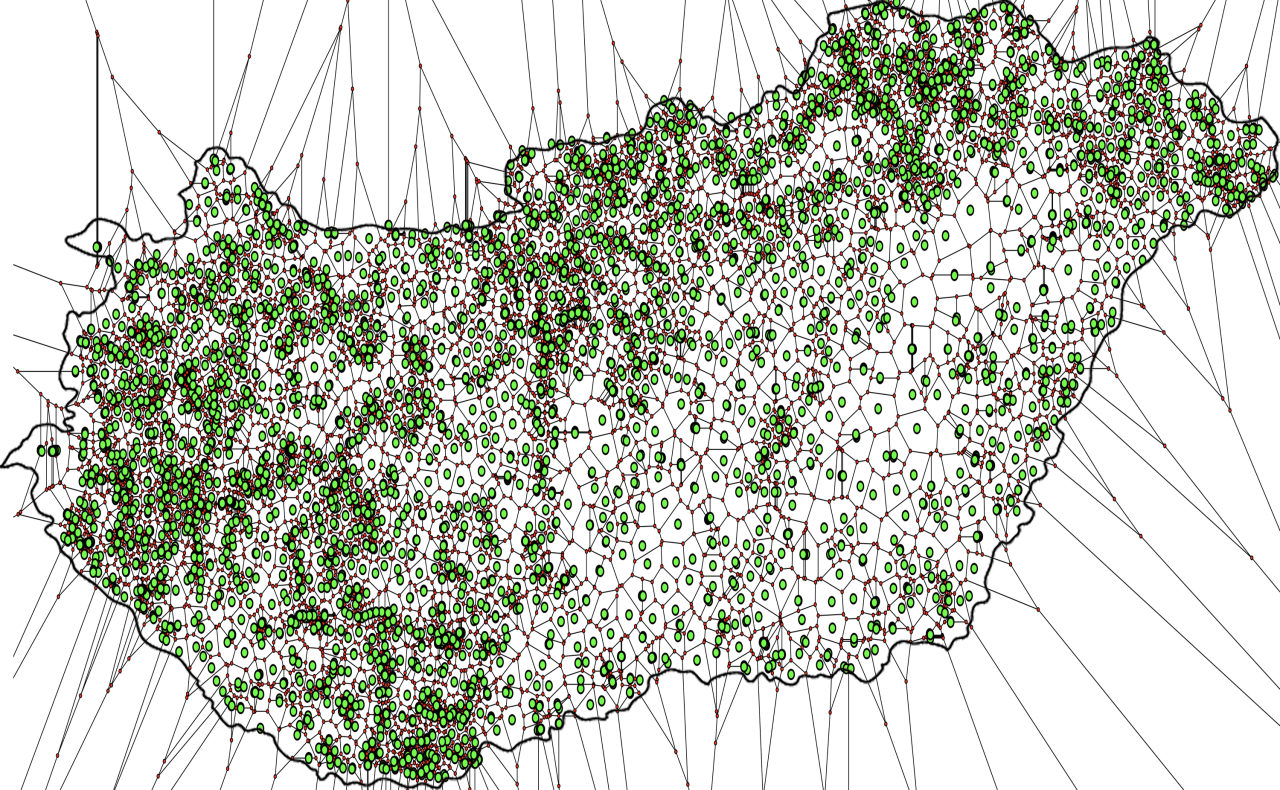
\includegraphics[width=\textwidth]{images/hungary_voronoi.png}
    \caption{Kossuth utcák Voronoj-diagramja Magyarország felett}
    \label{voronoj:hun}
\end{figure}

A \ref{voronoj:hun}. ábrán látható térképet nézegetve egyből szembetűnik, hogy a Tiszántúlon a ritkább népsűrűséghez ritkább Kossuth-koncentráció is tartozik. Naívan így azt gondolhatjuk, hogy az eredményt is majd ott kell keresni. Ha a fent leírt algoritmust lefuttatjuk, ténylegesen ott is fog nekünk eredményt találni, mégpedig a Hortobágyi Nemzeti Park környékén\footnote{Az algoritmus első futtatásakor Körösladány környékére tette az eredményt, azonban alapos vizsgálat kimutatta, hogy a város vasútállomásának bekötőútját a közelmúltban átnevezték Vasút utcáról Kossuth-ra, mely átnevezésről az OpenStreetMap nem tudott. Szerencsére, mivel az OSM adatbázisa bárki által szerkeszthető, ez a hiba azóta már orvosolva lett a szerző által}. Ez a pont azonban nem a legtávolabbi pont, mivel algoritmusunkba egy hiba csúszott.

\bigskip

Első éves hallgatóként anno megtanultuk, hogy az egyik leggyakoribb programozási hiba nem gondolni arra, mit csinál a programunk, vagy algoritmusunk az adatsorok határán. Bár általában ezt képletesen kell érteni (tömbök esetén például a tömb elején és végén érdemes megvizsgálni jól működik-e a programunk), itt azonban tényleges határról van szó: ha ügyesek vagyunk észrevesszük, hogy nemcsak a Tiszántúlon, hanem a határmenti területeken is ritkábbak a Kossuth utcák. Itt azonban algoritmusunk nem működik kielégítően, hisz az csak a Voronoj-cellák metszéspontját vizsgálta eredetileg. A hiba javításához a határmenti cellákra rá kell illesztenünk Magyarország határvonalát, és a kettő metszésében található pontokat is meg kell vizsgálnunk.

\bigskip

Az algoritmust újra lefuttatva megkapjuk a tényleges nyertest: a szlovén-osztrák-magyar hármashatár pontot. Innen a legközelebbi Kossuth utca úgy 17km-re található, Szentgotthárdon. Ha egy túra során el szeretnénk zarándokolni ide, a Kossuth utcáktól való félelmünkben, akkor örülhetünk, ugyanis ez a lokáció több okból is híres. Egyrészt hármashatár pont, másrészt ez Magyarország legnyugatibb koordinátája is. A helyszínen így egy kisebb pihenőt, játszóteret, valamint piknikezésre alkalmas padokat is találunk, hogy teljes mértékben kiélvezhessük túránk gyümölcsét. Azonban, ha egy kicsit nagyobb kihívásra vágyunk, a második helyen a Hortobágyi Nemzeti Park területén található ponton leszünk legmesszebb a Kossuth utcáktól, úgy 13km-re. Itt azonban nem lesz semmi indikátora a helyszín fontosságának, mindenképp érdemes egy jól feltöltött, és precíz GPS lokátorra hagyatkoznunk a célpont megtalálásához.

\bigskip

A teljes adatsor, valamint egyéb példák, mint például Petőfik, Rákóczyk vagy József Attilák megtekinthetők a projekt honlapján\cite{kossuthmap}, ahol kiderül, hogy Magyarországon bárhol is vagyunk lesz 12km-en belül egy sportlétesítmény, az Egyesült Királyságban meg nagy átlagban -- különösen Angliában -- ha véletlenszerűen ledobnak egy repülőből\footnote{remélhetőleg működő ejtőernyővel}, akkor 1km-en belül fogunk találni egy kocsmát. Ami jól jön ha esetleg egy kis frissítőre vágynánk a landolás után.

% ------------------------------------------------------------------------------

\section{A lombkoronák réme}

2023. év elején nagy port kavart egy hírhedt falétesítmény az ország keleti felén\cite{lombkorona}. Számos hírportál írt cikkeket, és vizsgálta az ügyet. Az Átlátszó adatvizualizációs csapata, az ATLO Team is készített a létesítményről egy inforgrafikát, melyet a \ref{atloteam:question}. ábrán látható felhívással tettek közre\cite{atloteam:tumblr}.

\bigskip

\begin{figure}[!htbp]
    \centering
    \BeginAccSupp{method=plain,Alt={Felmerült, hogy lehetne belőle egy FPS-t csinálni. Innen le lehet tölteni a 3D-modellt}}%
    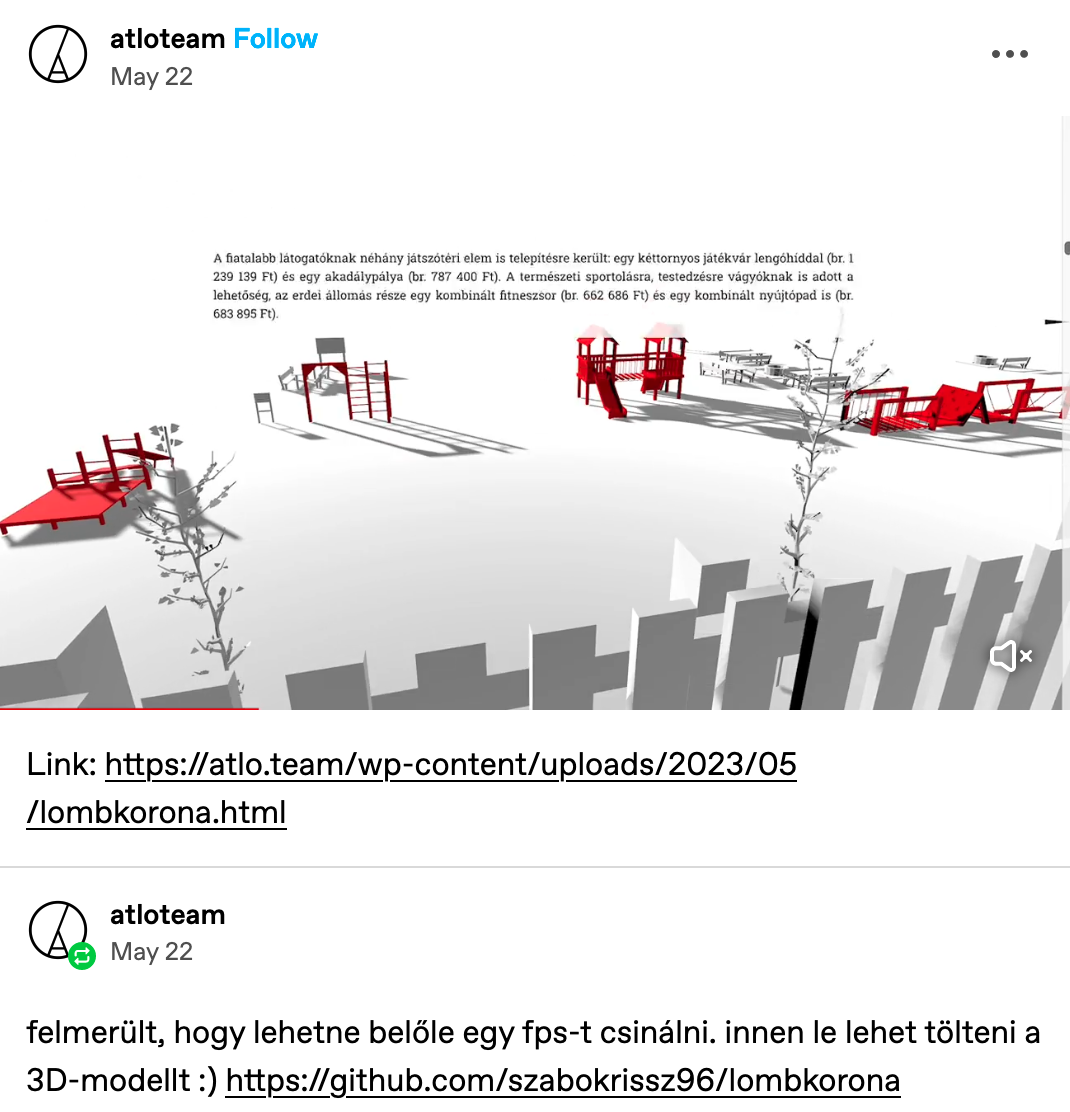
\includegraphics[width=\textwidth]{images/atlo_kerdes.png}
    \EndAccSupp{}%
    \caption{A problémafelvetés}
    \label{atloteam:question}
\end{figure}

Természetesen kaptam az alkalmon, hogy megnézzem mit is lehet egy ilyen modellel tenni! 3D grafikával volt némi kapcsolatom már középiskolai éveim során is, amikor megjelentek a korabeli webes 3D rendszerek, például a VRML. 2D alapú játékfejlesztés mindig is érdekelt, több 2D alkalmazás fejlesztésében is részt vettem, de 3D grafikával nem túl sokat foglalkoztam. Később, egyetemi éveim alatt bár jártam 3D grafikával foglalkozó extra kreditre, de szerintem csak azért sikerült azt teljesítenem, mert a vizsgán az első tételt húztam, ami bevezetésképpen csak két dimenziós terekkel foglalkozott.

\bigskip

Mindezt összevetve kíváncsivá tett mennyit fejlődött a technológia az elmúlt 25-30 évben, azóta amióta először találkoztam a VRML nagyon korai példányaival. Úgy rémlik már akkor is sikerült benne egy nagyon-nagyon kezdetleges FPS-t\footnote{Belső nézetű lövöldözős játékot} elkészítenem, bár sajnos már nincs ennek nyoma az archívumomban. Persze nem kell túl sokat gondolni: egy lapos szürke sík terep volt a talaj, és pár kockadarab jelezte a falakat rajta. Ellenfél nem volt, csak statikus gömbök (talán sárga színűek), amelyeket fel kellett venned. A falak pedig azt sem érzékelték ha nekimentél, simán át lehetett siklani rajtuk. Persze ne feledjük el, ez még bőven a múlt évezred végén volt, amikor még az Internet Explorer és a Netscape Navigator volt a két legismertebb böngésző, és sokan gondolták, hogy a honlapokon majd Java alapú alkalmazások fognak futni. Szerencsére azóta már se Internet Explorer, se Netscape Navigator, és a Java alapú alkalmazásokat is csak az APEH -- mai nevén NAV -- vette komolyan.

\bigskip

No de lássuk mennyi mindent fejlődött a világ úgy 25 év alatt: egy kis Google keresés kidobott egy Three.JS keretrendszer alatt írt FPS rendszert\cite{fpsdemo}, amiben csak a terepet kellett lecserélni a nyírmártonfalvi lombkoronasétány modelljére, és 5 perccel később már kész is volt egy nagyon kezdetleges, de működő játék. Lehetett benne mozogni, lőszert felvenni a földről, lövöldözni, a tereptárgyaknak neki lehetett menni (és nem siklottál át rajtuk), valamint az ellenfél is próbált némi intelligenciát mutatni azzal, hogy megpróbált üldözni, meg csapkodni. Bár természetesen a grafika nem egy AAA kategóriás játékot idézett, lényegesen jobban nézett ki, mint bármi más, amit pár perc alatt, webes platformra össze lehetett hozni, mondjuk úgy 10 éve.

\bigskip

Az igazán érdekes rész viszont csak ezután következett. Bár egy valamennyire működő játék 5 perc alatt elkészült, azért ez nem volt túl nagy teljesítmény, tekintve hogy csak más emberek által ekészített projekteket hoztam össze egy kalap alá. A Telex, akinek tudomására jutott a honlapom is elintézte az egész próbálkozást azzal, hogy ,,(csak) arról van szó, hogy valaki ráhúzta egy már létező kezdetleges, belső nézetes demóra a lombkoronasétány virtuális mását''\cite{telex}. Így írjon rólad szépeket a magyar média ugyebár. Pedig ők már a javított változatot látták, mert hát a projekt nem állt le, sőt most kezdett csak érdekessé válni az egész.

\bigskip

A rendszerben még volt bőven hiba, és mivel a játékmotort nem magam írtam, ezért ezek kijavításához először rá kellett jönni, hogy mi, hogyan, és miért úgy működik, ahogy. Szerencsére az eredeti kód nem volt túl komplex (bár nem is volt túldokumentálva), így sikerült hamar megfejteni a működésének alapjait, és a vizsgálgatás során lehetett tanulni egyet s mást a 3D grafika, valamint a játékfejlesztés alapjairól. A két nap, amit ebbe a projektbe fektettem, mindenképp többet tanított nekem, mint egy fél évnyi 3D grafika az egyetemen. Vagy lehet csak izgalmasabb volt!

\bigskip

Néhány példa, hogy miket sikerült ez alatt a pár napos fejlesztés alatt tanulnom:

\begin{itemize}
    \item A navmesh működése -- 3D modell ami megmutatja az AI által irányított lényeknek, hogy hova mehetnek, és hogyan jutnak oda a leggyorsabban
    \item Különféle textúrák működése webes környezetben, beleértve az égbolt és talaj rendes mintázatát
    \item Különféle ütközésvizsgálati módszerek, statikus-dinamikus illetve dinamikus-dinamikus modellek között
    \item Játéktechnikai javítások -- jobb AI kezelés, különféle nehézségi szintek, többfajta sebezési pontok támogatása
    \item Webes hangkezelés 3D térben, valamint a játék kezelésének támogatása mobil környezetben
\end{itemize}

Az elkészült projekt és a forráskód hozzá megtekinthető a szerző honlapján\cite{canopyfps}.

% ------------------------------------------------------------------------------

\section{Másfélmillió lépés Magyarországon, tömegközlekedve}

A 3D-s kitekintő után egy újabb térképészeti feladat az \ref{mfm:question}. ábrán, ezúton \texttt{mindenfoglaltmar} nevű felhasználótól\cite{kekkorkereso:tumblr}.

\begin{figure}[!htbp]
    \centering
    \BeginAccSupp{method=plain,Alt={Van-e valakinek ötlete olyan kék túra szakaszra, ami 15-20 km közötti és megközelíthető úgy, hogy A ponton hagyom a kocsit, eltömegközlekedek B pontra és visszasétàlok A pontba?}}%
    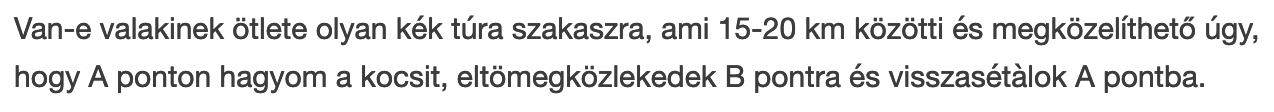
\includegraphics[width=\textwidth]{images/kekkor_kerdes.png}
    \EndAccSupp{}%
    \caption{Problémafelvetés}
    \label{mfm:question}
\end{figure}

\bigskip

Megint egy tökéletes feladat, ha esetleg túl sok határidős munkánk lenne, és egy kis agyi felfrissülésre vágynánk -- miközben természetesen segítünk valakinek megoldani világraszóló problémáját. A fenti feladat hasonlóan térképészeti megoldást igényel, mint a Kossuth térképes, azonban más forrásokból kell beszerezni hozzá az adatokat. Az ötlet az az, hogy megpróbáljuk megtalálni az összes létező kombinációját az olyan túráknak, amelyek egy buszmegállóból indulnak, eljutnak egy másik buszmegállóba tömegközlekedve, onnan egy rövid sétával továbbvisznek egy kéktúrás pecsételőhelyhez, majd onnan elvezetnek a kiszemelt Kéktúra szakaszon keresztül vissza abba a buszmegállóba, ahonnan eredetileg is indultunk. Nézzük honnan szerezzük be az adatokat ehhez.

\begin{itemize}
    \item Szükségünk lesz a Kéktúrák teljes útvonalára. Ez elérhető a Kéktúra hivatalos honlapjáról GPX formátumban. Az egyszerűség kedvéért a három különböző Kéktúra vonalát \texttt{QGis} segítségével kézzel összefűztem egyetlen Magyarországot átszelő Kékkörré
    \item Szükségünk lesz Magyarország összes buszmenetrendjére -- vagy legalábbis azokra, melyek Kéktúra szakaszok közelében helyezkednek el. Mind a BKK, mint a Volánbusz ezt az adatsort ingyenesen elérhetővé teszi bárki számára a honlapján, GTFS formátumban. A MÁV oldalán sajnos ez nem szerepel, de ezt nem tekintjük túl nagy problémának. A Budapest környéki vasútvonalak, például a HÉV menetrendek így is szerepelni fognak a rendszerben, a BKK adatbázisa miatt.
    \item Végezetül turistautat kell találnunk a buszmegállók és a Kéktúra szakaszok kiinduló és végpontjai között. Erre megint az OSM adatbázisát fogjuk hasznáni, onnan nyerjük ki a potenciális gyalogutakat.
\end{itemize}

Miután a nyers adatokat beszereztük, fel kell őket dolgozni. Először is minden, a Kéktúra szakaszok végpontjaihoz közel lévő buszmegállót összegyűjtünk. Az egyszerűség kedvéért az egymástól csak párszáz méterre lévő buszmegállókat egynek tekintjük, mivel általában ezek az út két szemközti oldalán helyezkednek el. Miután kiszűrtük a buszmegállókat, lefuttatunk egy keresést, ami megkeresi a legrövidebb turistautat a buszmegállók és a Kéktúra szakaszok végpontjai között. A szerző több különféle technológiát is kipróbált, végül az adatokat egy PostGIS\cite{postgis} adatbázisba töltötte be és a \texttt{pg\_routing} programcsomag segítségével kereste meg az eredményt, A* algoritmus segítségével.

\bigskip

A következő lépcsőfok a buszútvonalak kiderítése. A GTFS adatsort egy OpenTripPlanner\cite{opentripplanner} nevű programba töltjük be, ahonnan ezután lekérdezhetjük, hogy A és B pont között milyen útvonalak léteznek. Ezt a keresést szintén lefuttatjuk az összes buszmegállópár között (bizonyos távolsági kereteken belül), majd az eredményeket sorbarendezzük kritériumaink alapján, hogy megkapjuk az optimális buszmenetrendeket. Ilyen kritériumok például, hogy melyik a leggyorsabb, a legsűrűbb, vagy esetleg a legkevesebb átszállást, illetve gyaloglást igénylő útvonal.

\bigskip

Miután minden adat megvan már csak egy honlapot kell fejleszteni, ahol a három különböző szekciót egy térképen ábrázolunk, kereshető formátumban. Persze az eredeti kérdés csak a 15-20km-es szakaszokra vonatkozott, ha igazán hasznos honlapot szeretnénk készíteni gondolunk olyanokra is, akik ennél csak kevesebbet, vagy ellenkezőleg jóval többet szeretnének túrázni.

\bigskip

\begin{figure}[!htbp]
    \centering
    \BeginAccSupp{method=plain,Alt={Térkép, rajta egy turistaútvonal bejelölve a kéktúra Dobogókő és Kevély nyereg közötti szakaszának ábrázolásával}}%
    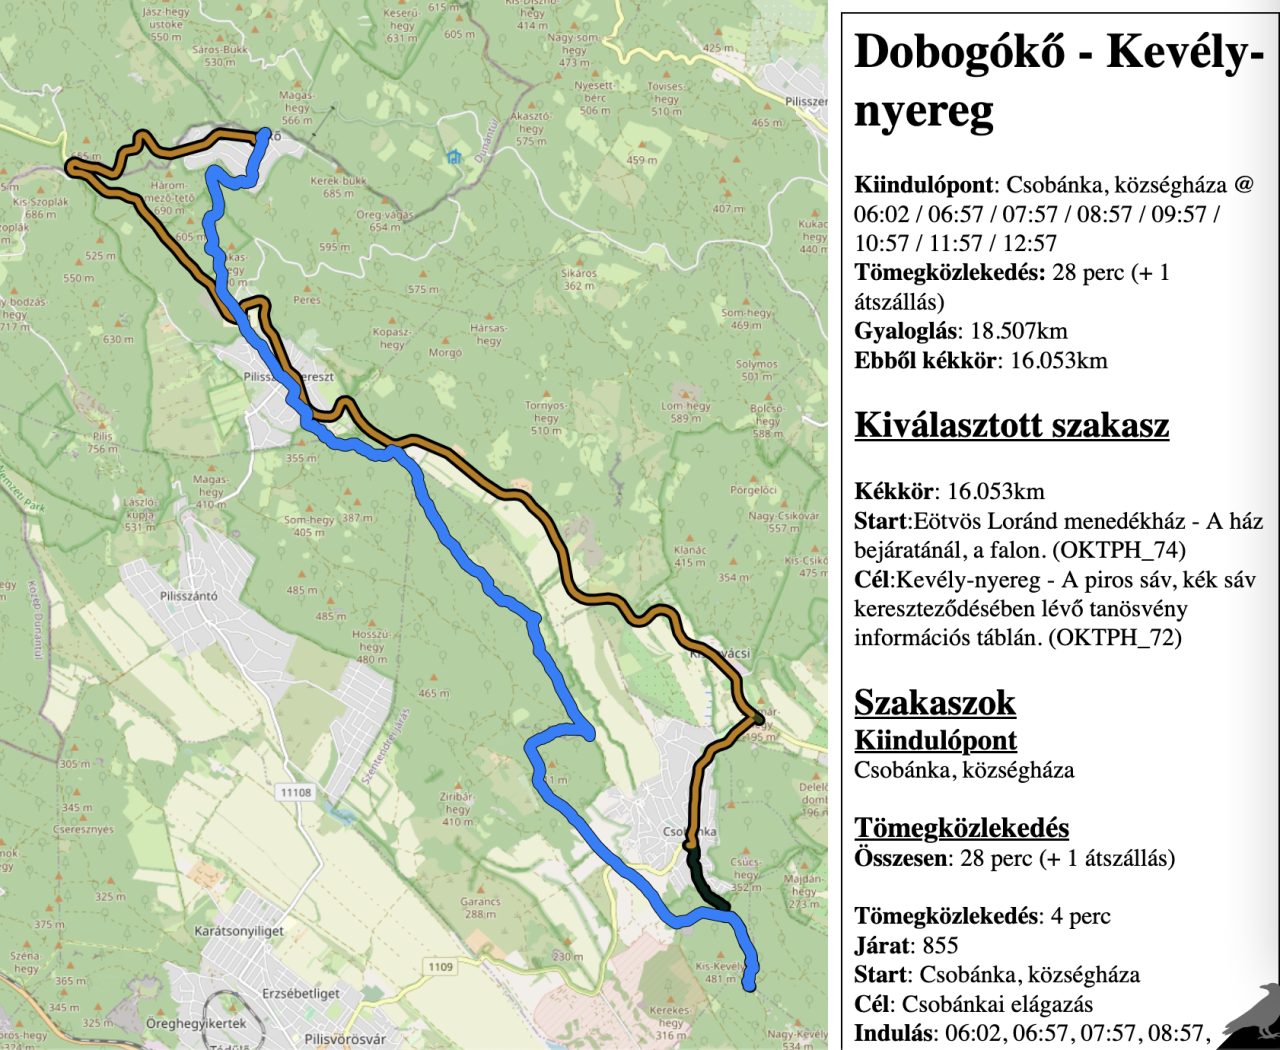
\includegraphics[width=\textwidth]{images/kekkor_results.png}
    \EndAccSupp{}%
    \caption{Dobogókő - Kevély nyereg túrajavaslat}
    \label{kekkor:answer}
\end{figure}

Mindenesetre az eredeti kérdésre a válasz: rengeteg ilyen útvonal létezik, Budapest környékén egyből három ilyen szakasz is van: A Dobogókő -- Kevély nyereg, a Piliscsaba -- Dorog, valamint a Mogyorósbánya -- Dorog szakasz mind bejárható egy nap alatt egy rövid kis 15-20km sétálással, de pár szakaszt leszámítva majdnem az egész Kékkör elvégezhető napi 20-25km sétálással úgy, hogy mindig visszajutunk a kiindulópontunkra a nap végén.

\bigskip

A Kékkör kereső alkalmazás és forráskódja szintén megtalálható a szerző honlapján\cite{kekkor:site}.

\section{Utószó}

Remélem a fenti pár példa meghozta az olvasók kedvét arra, hogy érdekes problémafelvetések megoldására új technológiákat próbáljanak ki, különösen ha azok amúgy nem tartoznak a nap-mint-nap használt eszköztárukba. Még ha nem is sikerül megoldani a problémát, rengeteget lehet tanulni a sikertelen kísérletekből is. És természetesen ne feledjünk, hogy nem csak furcsa kérésekkel lehet másokon segíteni, a bevezetőben említett szervezetek folyamatosan várják önkéntesek jelentkezését. Tanulni vágyó illetők mindig lesznek, és mindig lesz szükség arra, hogy valaki tanítsa őket. Ötleteket, új technológiákat, érdekes problémákat ezen alkalmak során is bőven lehet gyűjteni.

\bigskip

Ha sokáig csináljuk ezeket a projekteket, előbb-utóbb utolér a hírnév is, így könnyen lehet, hogy amikor valaki megkérdezi tőlünk, hogy ,,te, meg tudod mondani, hogy melyik az a busz, ami a legtöbb Kossuth utcán halad át'', és akkor erre már tudod is egyből a választ, hogy ,,természetesen, amit te keresel az a Nagykanizsa és Zalaegerszeg között közlekedő 6458-as busz, ami rekordmennyiségű, hét különböző Kossuth utcán is megáll, az egyiken kétszer is, a két végén''.

\bigskip

,,Hétköznap érdemes felszállni rá reggel 6:25-kor, Nagykanizsán.''

\bigskip

A szerzőnek számos más projektje is van, különösen szeret térképészeti problémákat megoldani és politikai indítattású játékokat készíteni. Portfóliója megtalálhatók a honlapján\cite{sztupy:projects}.

\begin{thebibliography}{99}

\bibitem{codebar} Codebar is a charity that facilitates the growth of a diverse tech community by running free regular programming workshops for minority groups in tech. \href{https://codebar.io}{\texttt{codebar.io}}

\bibitem{migracode} MigraCode Europe A European Network to promote Open Tech Education for Refugees and Migrants. \href{https://migracode.eu}{\texttt{migracode.eu}}

\bibitem{sztivan} Az észtek litvánok lettek, ID \#182822065158 \\
\href{https://sztivan.tumblr.com/post/182822065158}{\texttt{sztivan.tumblr.com/post/182822065158}}

\bibitem{osm} OpenStreetMap, a free, open geographic database updated and maintained by a community of volunteers via open collaboration. \\
\href{https://openstreetmap.org}{\texttt{openstreetmap.org}}

\bibitem{turistautak} turistautak.hu Magyarország leggyorsabban fejlődő nonprofit térkép-portálja
\href{https://turistautak.hu}{\texttt{turistautak.hu}}

\bibitem{voronoj} Wikipédia-szerkesztők, 'Voronoj-cella', Wikipédia, 2022. május 22. \\
\href{https://hu.wikipedia.org/w/index.php?title=Voronoj-cella&oldid=24947920}{\texttt{hu.wikipedia.org/w/index.php?title=Voronoj-cella}}

\bibitem{kossuthmap} Zsolt Sz Sz Raven, Determine furthest points away in a country for a specific set of points
\href{https://sztupy.hu/kossuth-map/}{\texttt{sztupy.hu/kossuth-map}}

\bibitem{lombkorona} Sokszínű Vidék, Kivágott erdő helyén épült lombkorona-sétány Nyírmártonfalván \\
\href{https://sokszinuvidek.24.hu/mozaik/2023/03/23/lombkorona-setany-nyirmartonfalva-nyirseg-hajdu-bihar-megye-erdo/}{\texttt{sokszinuvidek.24.hu/mozaik/2023/03/23/lombkorona-}$\curvearrowright$\\\texttt{setany-nyirmartonfalva-nyirseg-hajdu-bihar-megye-erdo}}

\bibitem{atloteam:tumblr} ATLO Team, powered by ATLATSZO. ID \#718041277567025152 \\
\href{https://atloteam.tumblr.com/post/718041277567025152}{\texttt{atloteam.tumblr.com/post/718041277567025152}}

\bibitem{fpsdemo} Mohsen Heydari, Three FPS Demo \\
\href{https://github.com/mohsenheydari/three-fps}{\texttt{github.com/mohsenheydari/three-fps}}

\bibitem{telex} Flachner Balázs, Virtuálisan ugyan, de már mutánsokra is lehet lövöldözni a lomb nélküli lombkoronasétánynál\\
\href{https://telex.hu/zacc/2023/05/24/lombkoronasetany-nyirmartonfalva-videojatek-lovoldozes}{\texttt{telex.hu/zacc/2023/05/24/lombkoronasetany-}$\curvearrowright$\\\texttt{nyirmartonfalva-videojatek-lovoldozes}}

\bibitem{canopyfps} Zsolt Sz Sz Raven, Canopy FPS \href{https://sztupy.hu/lombkorona/}{\texttt{sztupy.hu/lombkorona}}

\bibitem{postgis} PostGIS extends the capabilities of the PostgreSQL relational database by adding support storing, indexing and querying geographic data.
\href{https://postgis.net/}{\texttt{postgis.net}}

\bibitem{opentripplanner} OpenTripPlanner (OTP) is a family of open source software projects that provide passenger information and transportation network analysis services. \\
\href{https://opentripplanner.org/}{\texttt{opentripplanner.org}}

\bibitem{kekkorkereso:tumblr} SztupY, ID \#728193481495003136 \\
\href{https://tumblr.sztupy.hu/post/728193481495003136}{\texttt{tumblr.sztupy.hu/post/728193481495003136}}

\bibitem{kekkor:site} Zsolt Sz Sz Raven, Kékkör szakasz kereső \\
\href{https://sztupy.hu/kekkor-kereso/}{\texttt{sztupy.hu/kekkor-kereso}}

\bibitem{sztupy:projects} Zsolt Sz Sz Raven, Projects page \href{https://sztupy.hu/projects/}{\texttt{sztupy.hu/projects}}

\end{thebibliography}


\end{document}
